\chapter{Annotation Service}

\section{Objective of the Annotation Service}
As described in 2.4.2, the goal of the AS is to provide a user with the possibility to:
\begin{enumerate}[(1)]
	\item view A WSI
	\item annotate a WSI
	\item manage made annotations
\end{enumerate}

In order to achieve objective (1) - (3), a GUI needs to be deployed which supports the user in working on those tasks. (3) also adds the need for file persistence management.


\section{Methodology}
As stated in 2.1, most vendors have proprietary image formats and their own implementation of a viewer for those, thus creating a vendor lock-in. Further do vendors often only support Windows platforms, ignoring other operating systems\cite{Cornish13}\cite{DICOM10}\cite{Farahanil15}. To avoid this, a solution must be found that is independent of operating system and vendor.

Chap. 3 already established a service to convert WSIs of various formats into the DZI format, solving the problem of multiple proprietary formats. 

Independence from an operating system can be achieved by using web technologies, especially when running an application in a web browser\cite{Tseytlin14}, since those are supported by all modern operating systems. 

Because of this, the AS will be implemented as a web browser application. 


\subsection{Functionality of the Annotation Service}
The goal of viewing a WSI (1) is a straight forward task. (2) and (3) are more elusive. For that reason, this subsection elaborates on the functionality needed to help achieve those objectives.

Annotations will be created by drawing directly onto the viewed WSI. If the user spots a region of interest, a contour can be drawn around it. This can  either be done in \emph{free hand} or \emph{polygon mode}. In free hand mode, the contour will be drawn along the path of the mouse pointer, until the mode is disabled again. Upon deactivation, the contour will be closed. In polygon mode, the user can place coordinates which will be connected from one to another in the order they're placed in. A contour in this mode considers to be closed, once a point on the contour is clicked a second time. A marked region of interest is simply called \emph{region} from this point on.

The information what a region is surrounded by can be as valuable as the information about the region itself\cite{Bankman00}. Therefore, every region will have a \emph{context} trait, which lists every label of regions it touches, crosses, surrounds or is surrounded by (see fig. \ref{fig4_contextregions}).

\begin{figure}[H]
	\begin{center}
		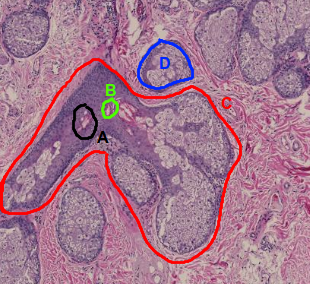
\includegraphics[scale=0.8]{img/contextregions.png}
		\caption{Example of context regions (B, C are context of A; A, C are context of B; A, B are context of C; D has no context region)}
		\label{fig4_contextregions}
	\end{center}
\end{figure}
% TODO: add figure about context regions

Another way of creating regions will be so called \emph{points of interest} (POI)\nmc{POI}{Point of Interest}. A POI will be placed with a mouse click. After that, an external script will be invoked to run an automated segmentation in the proximity of the POI and return with a contour which will be marked as region. The segmentation approaches may differ drastically in different scenarios\cite{Liu12}, therefore the script will be interchangeable\footnote{There are many different ways of how to approach the topic of segmentation (e.g. \cite{Qi12}, \cite{Sharma16}, \cite{Wienert12}, \cite{Angulo10} for cell segmentation alone). Writing a fully working segmentation script is worth another thesis by itself, therefore only a dummy implementation will be delivered with this work.}.

Each region has a \emph{label} associated to it. A label is a predefined string, which describes what the region just created shows. The labels available will be determined through a \emph{label dictionary}, which is a container that offers a list of strings to select from. This approach guarantees a unified labeling, independent of a specific WSI or pathologist. The option to choose between multiple available label dictionaries opens up the possibility of creating dictionaries which are specialized on certain cases or studies. Again, to keep up labeling integrity, labels can only be selected from one dictionary per WSI.

Users will be able to create new, empty dictionaries, if the need arises. Furthermore, they will be able to add entries to existing and new dictionaries alike, to further advance or specialize them. To delete single entries or whole dictionaries, file access to the server is necessary. This is due to the fact, that knowledge can by added without direct negative consequences. Deleting existing knowledge influences all WSIs on which this knowledge was used, may it be as a label or a whole dictionary.

To support the user in annotating a WSI, a distance measurement tool will be usable as well. This tool can measure the distance between 2 pixels in $\mu$m.


\subsection{Parts of the Annotation Service}
The AS is implemented in 2 parts. Those are the Annotation Service Server (ASS)\nmc{ASS}{Annoation Service Server} and the Annotation Service Viewer (ASV)\nmc{ASV}{Annotation Service Viewer}.

This is because of the \emph{same-origin policy} (SOP)\nmc{SOP}{same-origin policy}. SOP is a security concept of the web application security model. It prevents a direct access to files, if the parent directory of the originating file is not an ancestor directory of the target file\cite{web:mdn}. Because of the SOP, WSIs would have to be located in the directory structure of the AS, which by itself doesn't create a problem. To get a new WSI there, however, the user would be forced to navigate through the structure of the AS, find the correct directory and then place it there manually. This makes knowledge of the service structure necessary and creates a horrible UX. Furthermore, tinkering with the file structure of the AS creates a possible source for errors.

A workaround of this problem is to deploy a web server, which can redirect the image request, access the WSI and return it in response\cite{Tseytlin14}. The use of DZI creates another advantage: the used image pyramid model reduces the network traffic necessary to load and show a WSI in a viewer\cite{Cornish13}\cite{DICOM10}.

Furthermore, even a single WSI takes up a lot of storage capacity\cite{Singh11}. Having multiple WSIs on a local hard drive would either create the need for huge amounts of available storage space or restrict the amount of accessible WSIs to a few at any given time. The latter solution would create two follow-up problems:
\begin{itemize}
	\item WSIs are medical images and as such confidential information. Therefore, not everyone is allowed to just have access to or copies of them\cite{COA}\cite{USSanDiego}. Once a copy of a WSI changes hands, it is virtually impossible to make sure that privacy regulations will be uphold.	
	\item With only a small amount out of all WSIs accessible at all times, the need for copying files back and forth arises as soon as the user wants to compare, update or correct a WSI, which is not on his local file system at the given moment. Not only is this a great source for possible errors, but also very time consuming and inefficient.
\end{itemize}

With the use of a web server as a central image repository, WSIs and the access to them can be managed in a centralized spot, while upholding confidentiality regulations. Furthermore, a user has access to all of her/his WSIs at any given time, without the need for creating subsets and copying files back and forth. Depending on the setup of the network, other factors can come into play as well. Access to and sharing of rare cases, educational material and training samples can be granted without a complicated distribution chain and a smaller risk for confidentiality issues. It also enables the consultation of case experts independent of their physical position on the planet\cite{Wilbur09}.


\subsubsection{Annotation Service Server}
The ASS has 2 main purposes.

First, it serves as a so called \emph{Digital Slide Repository} (DSR)\nmc{DSR}{Digital Slide Repository}. A DSR manages storage of WSIs and their metadata. Additionally, it serves requested image data to a viewer client\cite{Cornish13}, such as the ASV. 

Second, it is responsible for file management. In detail, this means:
\begin{itemize}
	\item persist made annotations in a file
	\item deliver annotation data together with image data
	\item serve list of all available label dictionaries
	\item serve label dictionary entries
	\item save added entries to existing label dictionary
	\item create new, empty label dictionaries
\end{itemize} 

The development of a fully functional web server isn't in the scope of this thesis. Therefore, the ASS will run as a local web server. This works around many of the common issues when hosting a web server\cite{web:typicalissues}, such as:

\begin{itemize}
	\item inefficient data or page caching
	\item firewall throughput
	\item internet access throughput
	\item load balance issues
	\item gateway issues
	\item poor security design
	\item connectivity issues
\end{itemize}


\subsubsection{Annotation Service Viewer}
The ASV is developed to deploy a GUI through which the pathologist is enabled to view a WSI and annotate it. The ASV is developed in an iterative approach with the help of selected pathologists. After each iteration, the GUI and user experience (UX)\nmc{UX}{User Experience} will be evaluated. This way, the ASV can be adapted to the needs of a real life environment based on the pathologists feedback.

\begin{figure}[H]
	\begin{center}
		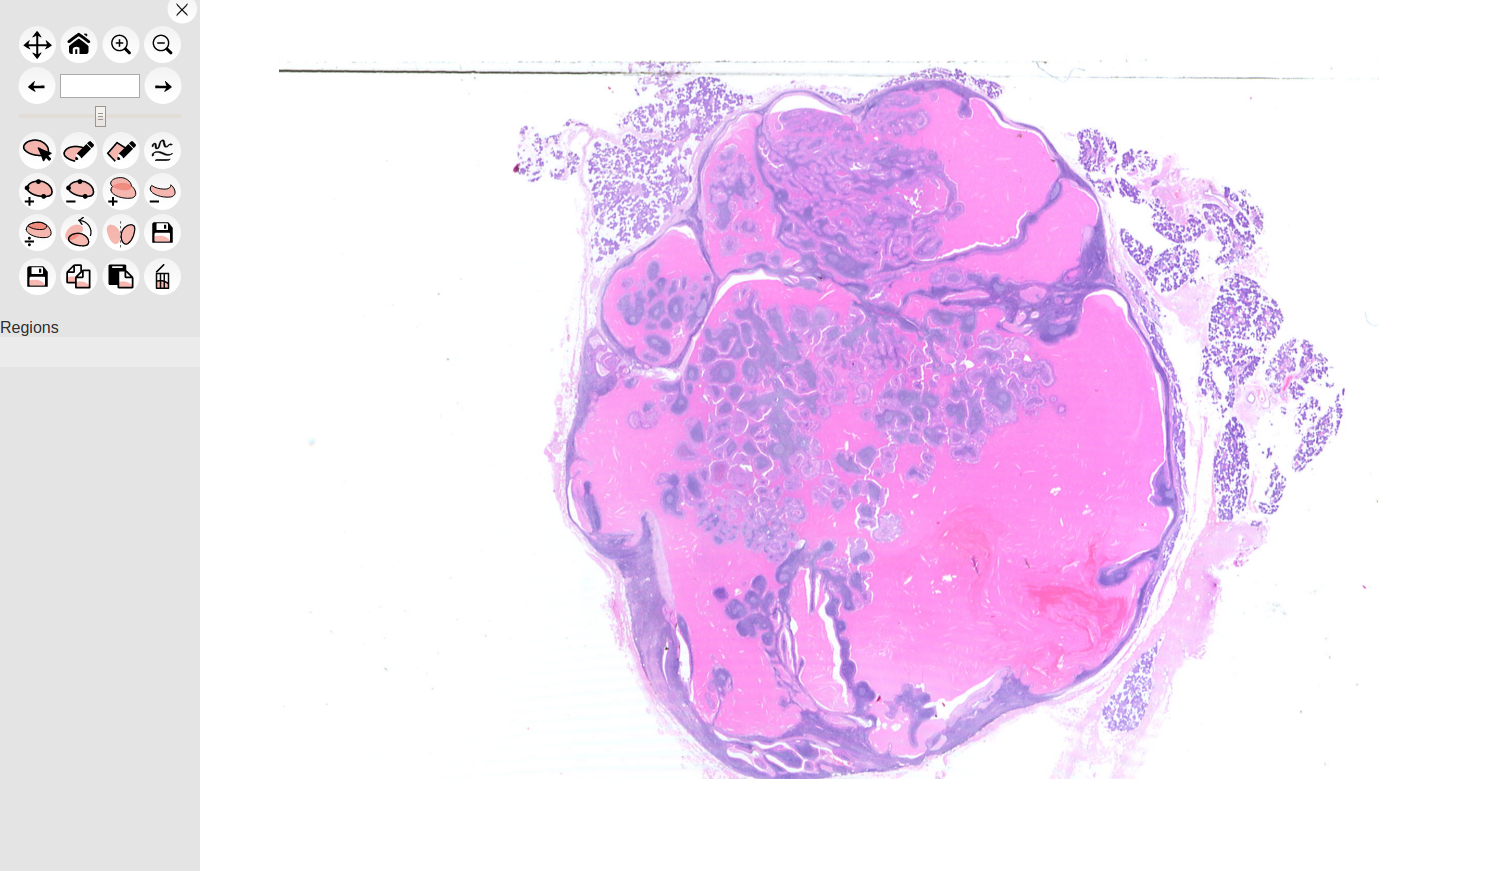
\includegraphics[scale=0.2]{img/microdrawUI.png}
		\caption{Microdraw GUI with opened WSI}
		\label{fig4_microdrawUI}
	\end{center}
\end{figure}

The first iteration of the ASV will be based on an open source project called \emph{MicroDraw}\footnote{See \url{https://github.com/r03ert0/microdraw} for more information on the MicroDraw project} (see fig. \ref{fig4_microdrawUI} for MicroDraws GUI).  MicroDraw is a web application to view and annotate \emph{"high resolution histology data"}\cite{web:microdraw2}. The visualization is based on another open source project, called \emph{OpenSeadragon}\cite{web:openseadragon}. Annotations are made possible by the use of \emph{Paper.js}\footnote{see \url{http://paperjs.org/} for more information on Paper.js}. This delivers a baseline for the functionality specified in 4.2.1 and can be further adjusted to the needs of the ASV.

Apart from the frameworks used, MicroDraw is written in JavaScript using HTML5, CSS3 and jQuery\footnote{see \url{https://jquery.com/} for more information on jQuery}.


\section{Implementation}
The AS was realized in 2 components: the ASS and the ASV. The implementation of the ASS was done in python with the use of \emph{OpenSlide} and \emph{Flask}. The ASV was implemented using JavaScript, HTML5 and CSS3 with the use of \emph{OpenSeadragon}, \emph{jQuery} and \emph{Paper.js}.

The following subsections will explain the implementation and used frameworks of the ASS (see 4.3.1) and the ASV (see 4.3.2), as well as the way how those 2 components work together (see 4.3.3).

For a detailed explanation of the single functions of ASS and ASV, see Appendix B.

% openslide, openslide web server
% python web server, flask, openslide, java script, html5, css, jquery
\subsection{Annotation Service Server}
To make OpenSeadragon capable of viewing it anyway, OpenSlides \emph{DeepZoomGenerator} (DZG)\nmc{DeepZoomGenerator} is used.
% openslide
% flask
% how does it work?
% where does it listen?
% functions?
% uses json to save annotations and dictionaries
% internal structure

\subsection{Annotation Service Viewer}
% paper
% osd
% jquery
% functions?
% loading process
% inizialization of paper and openseadragon

\subsection{Communication between Server and Viewer}

The communication between Server and Viewer is realized by Flasks \emph{route() decorator} (see fig. \ref{fig4_routeDecorator}), which binds a URL to a function\cite{web:flask}. When bound, the function will be called, once the specified URL is requested by the client.

\begin{figure}[H]
	\begin{center}
		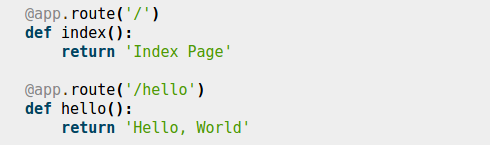
\includegraphics[scale=0.5]{img/route.png}
		\caption{Hello, World! example on how to use Flasks route() decorator (source: \cite{web:flask})}
		\label{fig4_routeDecorator}
	\end{center}
\end{figure}

A bound URL can also contain variable sections, which are marked as \emph{/{\textless}variable name{\textgreater}}. Optionally, a converter can by used to only accept variables of a certain type. This becomes possible by specifying the converter in front of the variable: \emph{/{\textless}converter:variable name{\textgreater}}\cite{web:flask}. See tab. \ref{tab4_converter} for the list of available converters in Flask.

\begin{table}[H]
	\begin{center}
		\begin{tabular}{| l | l |}
			\hline
			\textbf{name} & \textbf{accepted input}\\ \hline
			string & any text without a slash (default)\\ \hline
			int & integer values\\ \hline
			float & floating point values\\ \hline
			path & like string, but also accepts slashes \\ \hline
			any & matches one of the items provided\\ \hline
			uuid & UUID strings\\ \hline
		\end{tabular}
		\caption{Available converters in Flask (source: \cite{web:flask})}
		\label{tab4_converter}
	\end{center}
\end{table}

To bind a URL with one or more variable sections to a function, the corresponding function must have the variable sections as parameters:

\begin{lstlisting}[frame=single]
@app.route('/<slug>_files/<int:level>/<int:col>_
	<int:row>.<format>')
def tile(slug, level, col, row, format): ...
\end{lstlisting}

HTTP knows different methods for accessing URLs. By default, a route only answers to GET requests and refuses every other kind with a 405 HTTP status code. This can be changed by adding the \emph{methods} argument to the route() decorator (see fig. \ref{fig4_methods})\cite{web:flask}.

\begin{figure}[H]
	\begin{center}
		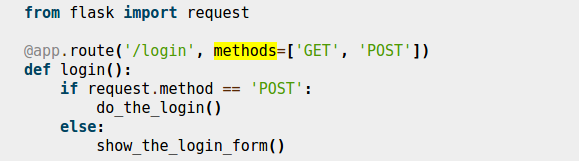
\includegraphics[scale=0.5]{img/HTTPmethods.png}
		\caption{Example use of the method argument (source: \cite{web:flask})}
		\label{fig4_methods}
	\end{center}
\end{figure}

The route() decorators used for communication between ASS and ASV are listed below. They first state their URL, then the bound function and parameter (\textbf{URL:} \emph{function(parameter)}), followed by a brief description of their functionality:

\begin{enumerate}[(1) -]
	\item\textbf{@app.route('/wsi/{\textless}path:file{\textunderscore}path{\textgreater}.dzi'):} \emph{index{\textunderscore}dzi(file{\textunderscore}path)}\\
	This URL is used to request a viewer with a specified DZI from the ASS. The ASS then renders an ASV and passes the path (\emph{file{\textunderscore}path}) to the DZI, its microns per pixel (MPP)\nmc{MPP}{Microns per Pixel} and its name to it. The ASV feeds the path to OpenSeadragon, which then views the DZI. The MPP are used to calculate the actual image size in $\mu$m for the scale. Lastly, the file name is used to change the name of the browser tab accordingly.
	
	\item \textbf{@app.route('/wsi/{\textless}path:file{\textunderscore}path{\textgreater}'):} \emph{index{\textunderscore}wsi(file{\textunderscore}path)}\\
	Works similar to (1), except that the requested image is not of the DZI format. To view it in OpenSeadragon anyway, an instance of the DZG is created which wraps the proprietary WSI. Then, a specific path ("\emph{/slide.dzi}") is handed to the ASV.
	
	\item \textbf{@app.route('/{\textless}slug{\textgreater}.dzi'):} \emph{dzi(slug)}\\
	Once the ASV requests slide.dzi, the DZG builds a response with the descriptive DZI file, created from the proprietary WSI format (via its \emph{.get{\textunderscore}dzi(format)} function, with \emph{format} being the file format of the tiles) and serves it to the ASV.
	
	\item \textbf{@app.route('/{\textless}slug{\textgreater}{\textunderscore}files/'\\{\textless}int:level{\textgreater}{\textunderscore}{\textless}int:col{\textgreater}{\textunderscore}{\textless}int:row{\textgreater}.{\textless}format{\textgreater}):}\\ \emph{tile(slug, level, col, row, format)}\\
	If an original DZI is requested, there is a \emph{/wsi/} in front of the URL. Therefore, this URL only triggers if (3) was called before. This way OpenSeadragon requests the separate tiles needed to fill the current view of the user. This is done via the DZG \emph{.get{\textunderscore}tile(level, address)} function. \emph{Level} describes the requested level, while \emph{address} is a tuple with the x (col) and y (row) position of the requested tile.
	
	\item \textbf{@app.route('/saveJson', methods=['POST']):} \emph{saveJson()}\\
	This URL is used when the user wants to save made annotations. The name of the JSON file and the content to write into it will be send via the POST request. The content of the POST request can be accessed via Flasks \emph{Request} object\cite{web:flask} in the following fashion:
	\begin{lstlisting}[frame=single]
post_data = request.form
source = post_data.get('file', default='')
content = post_data.get('content', default='{}').
	encode('utf-8')
	\end{lstlisting}
	
	\item \textbf{@app.route('/loadJson'):} \emph{loadJson()}\\
	(6) is used to load a JSON file, may that be the \emph{configuration.json}, a dictionary or saved annotations. The name of the source is passed as parameter (?src=[file]) to the ASS. Similar to (5), it can be accessed with the Request object\cite{web:flask}: \emph{request.args.get(parameter, default value)}.
	
	\item \textbf{@app.route('/createDictionary'):} \emph{createDictionary()}\\
	If the user sends the command to create a new dictionary, this URL is called. The ASS then creates a new, empty dictionary file. The name of the dictionary is passed as a URL parameter (?name=[name]) and then acquired in the same fashion as in (5). The ASS also opens the configuration file and changes the currently selected dictionary to the newly created one.
	
	\item \textbf{@app.route('/getDictionaries'):} \emph{getDictionaries()}\\
	When called, the ASS looks up the content of its \emph{dictionaries} folder and returns a list with the found file names or -1 in the case of an error.
\end{enumerate}